% =====================================================================
\section{결과: Regime Map}
\label{sec:results}
% =====================================================================

본 절의 RE10K 결과는 C1-a 본 실험(30-scene $\times$ view 수 $\times$ 예산 $\times$ \{MVSplat, Vanilla3DGS $\times$ 2 seed, FSGS $\times$ 2 seed\}, 2026-08-15 완료, 총 2400개 결과 셀 전량 확보)의 view 수 $\times$ 예산 축 전체를 반영한다.

overlap 축은 co-visibility selector 검증만 끝난 상태로 별도 실행이 필요하며, 보조 데이터셋 DL3DV는 착수 직후라 이번 판에는 포함하지 않는다(완료 후 갱신).

\subsection{품질--시간 Regime Map}

\begin{table}[h]
\centering
\caption{View 수 $\times$ 계산 예산별 승패 판정(RE10K 30-scene, 식~\eqref{eq:wtl}의 $\tau$ 적용). FF=MVSplat 우세, OPT=해당 optimization 방법 우세, Tie=$|\Delta| \le \tau$.}
\label{tab:regime}
\begin{tabular}{@{}l cccc@{}}
\toprule
View 수 & 1\,s & 10\,s & 60\,s & 300\,s \\
\midrule
\multicolumn{5}{@{}l}{\textit{Vanilla3DGS vs.\ MVSplat}} \\
2  & FF & FF & FF & FF \\
4  & FF & FF & FF & FF \\
8  & FF & FF & FF & FF \\
12 & FF & OPT & FF & OPT \\
\midrule
\multicolumn{5}{@{}l}{\textit{FSGS vs.\ MVSplat}} \\
2  & FF & FF & FF & FF \\
4  & FF & FF & FF & FF \\
8  & FF & Tie & OPT & OPT \\
12 & FF & OPT & OPT & OPT \\
\midrule
\multicolumn{5}{@{}l}{\textit{FSGS vs.\ Vanilla3DGS}} \\
2  & V3DGS & V3DGS & V3DGS & V3DGS \\
4  & V3DGS & V3DGS & FSGS & Tie \\
8  & Tie & FSGS & FSGS & FSGS \\
12 & Tie & FSGS & FSGS & FSGS \\
\bottomrule
\end{tabular}
\end{table}

\begin{figure}[h]
\centering
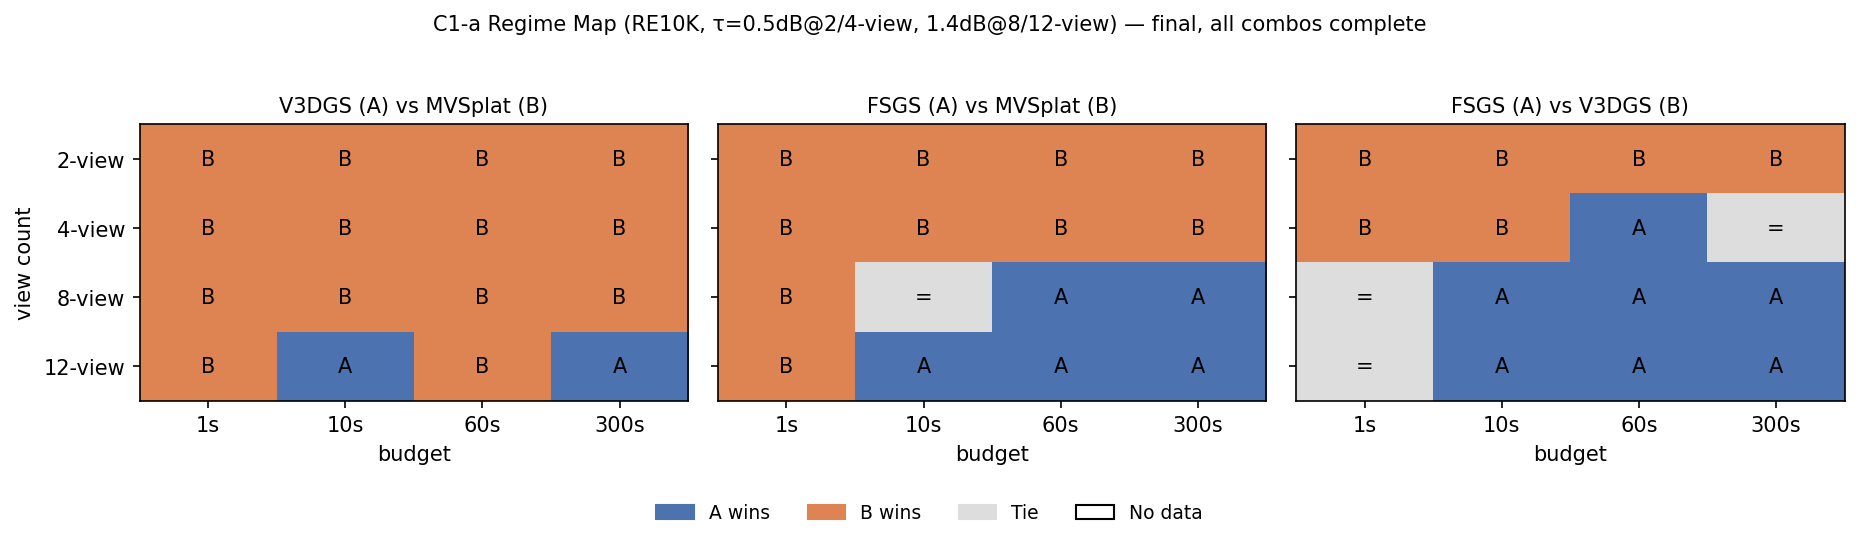
\includegraphics[width=\linewidth]{figures/regime_map.png}
\caption{품질--시간 Regime Map(RE10K 30-scene). 세 방법 쌍(Vanilla3DGS-vs-MVSplat, FSGS-vs-MVSplat, FSGS-vs-Vanilla3DGS) 각각에 대해 $\tau$ 적용 승패 판정(식~\eqref{eq:wtl})을 view 수 $\times$ 예산 격자로 표시. 표~\ref{tab:regime}과 동일한 데이터의 시각화.}
\label{fig:regime-heatmap}
\end{figure}

\subsection{품질--시간 Pareto frontier}

\begin{figure}[h]
\centering
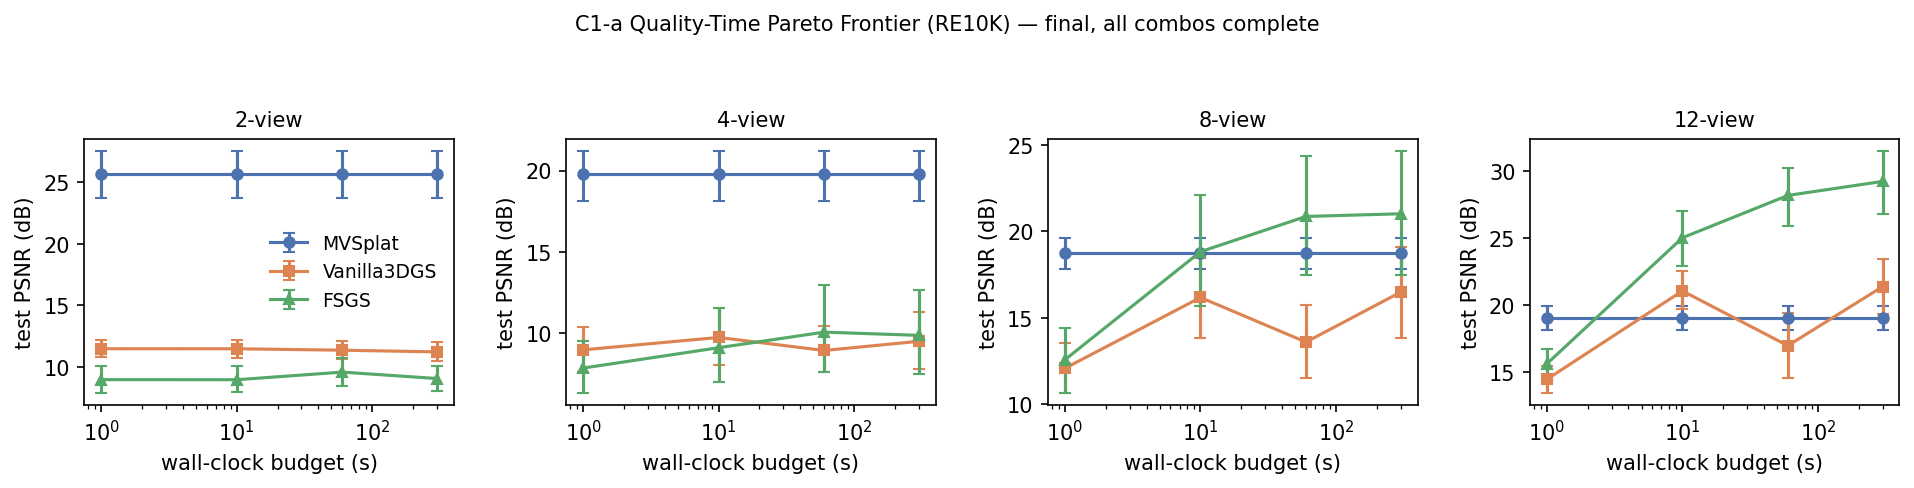
\includegraphics[width=\linewidth]{figures/pareto_frontier.png}
\caption{View 수별(2/4/8/12) 품질--시간 Pareto frontier(RE10K 30-scene). x축 예산(log scale, 1--300s), y축 test PSNR, 오차 막대는 scene cluster bootstrap 95\% CI.}
\label{fig:pareto}
\end{figure}

\subsection{장면별 win rate와 신뢰구간}

표~\ref{tab:regime}의 판정 중 두 지점은 신뢰구간까지 함께 보면 해석이 갈린다.

첫째, FSGS-vs-MVSplat의 8-view 역전은 예산이 늘수록 명확해진다. 60\,s에서 FSGS $20.85$\,dB(95\% CI $[17.48, 24.32]$) 대 MVSplat $18.71$\,dB($[17.79, 19.60]$), 300\,s에서는 FSGS $21.00$\,dB($[17.48, 24.64]$) 대 MVSplat $18.71$\,dB로, 두 CI가 겹치기는 하나 $\Delta$가 $\tau=1.4$\,dB를 넘게 유지되며 scene 수를 30개로 채운 뒤에도 방향이 뒤집히지 않았다(30-scene 이전 부분 데이터에서는 이 경계가 예산에 따라 판정이 흔들렸던 지점이었다).

둘째, 12-view에서 Vanilla3DGS는 예산에 대해 단조롭지 않다 — 10\,s에서 $21.06$\,dB로 MVSplat($19.06$\,dB)을 앞서지만 60\,s에서 $16.97$\,dB로 떨어졌다가 300\,s에 $21.38$\,dB로 회복한다. 이 60\,s 지점의 CI($[14.54, 19.45]$)는 MVSplat의 CI($[18.14, 19.93]$)와 크게 겹쳐 판정 자체는 유지되지만, pooled 평균만으로는 이 비단조성이 개별 scene의 학습 불안정(예: densification/opacity reset 주기와 예산 경계의 우연한 정렬)에서 오는지 체계적 현상인지 구분되지 않는다 — 원인 분석은 \S\ref{sec:failure}에서 다룬다.

\subsection{정성적 비교}

\begin{figure}[h]
\centering
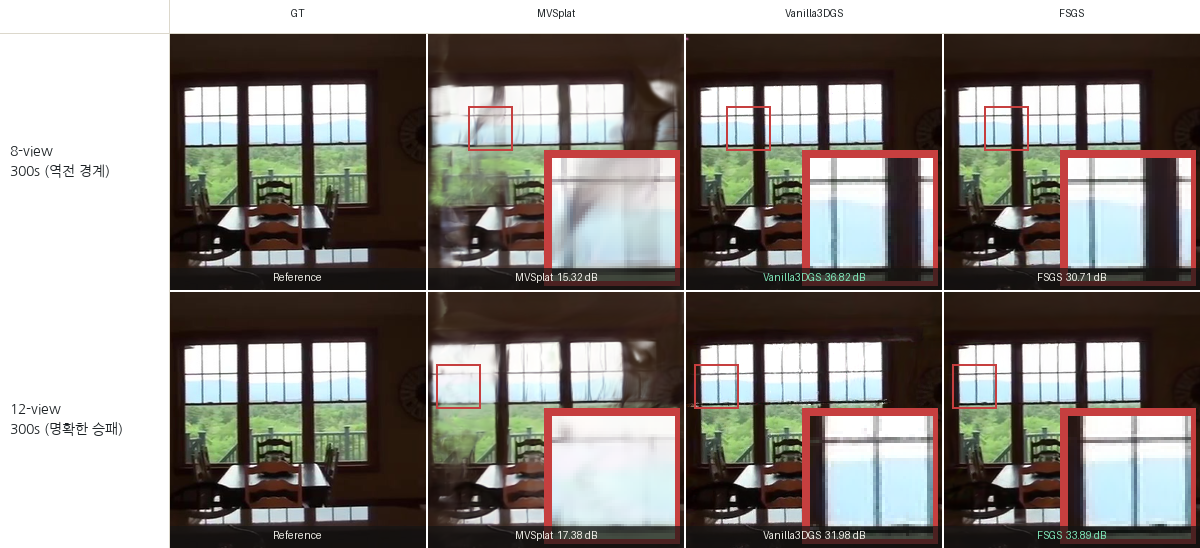
\includegraphics[width=\textwidth]{figures/qualitative_comparison.png}
\caption{RE10K scene \texttt{0588138dfec165a1}에서의 정성적 비교, 왼쪽부터 GT, MVSplat, Vanilla3DGS, FSGS(budget=300\,s). 위 행은 8-view(FSGS-vs-MVSplat 역전 경계 근방, \S\ref{sec:results}), 아래 행은 12-view(FSGS가 명확히 앞서는 조건). 각 패널 하단은 해당 target view의 PSNR(최고값은 초록색), 빨간 박스는 확대 영역(창틀 디테일)이다. MVSplat은 2-view 전용 학습이라 8/12-view 모두 분포 밖(OOD)이며 창틀이 흐릿하게 뭉개지는 것이 확대 영역에서 뚜렷이 보인다 — Vanilla3DGS/FSGS는 두 조건 모두 창틀 선이 살아있고 GT에 훨씬 가깝다.}
\label{fig:qualitative}
\end{figure}

\subsection{동일 초기값 Refinement On/Off}
\label{sec:c1b}

\todo{Feed-forward 출력을 고정한 뒤 refinement off(0\,s)/on(10/60/300\,s) 비교. 렌더 등가성 gate(\S\ref{sec:equivalence}) 통과 조건에서만 진행. 30-scene 최종 설정으로 재실행 필요.}

\subsection{확장 비교: Recurrent Refinement (ReSplat)}
\label{sec:resplat-exploratory}

이 비교군은 사전 등록 설계에 포함되지 않았으며 탐색적 결과로 서술한다. ReSplat~\cite{xu2026resplat}은 DepthSplat과 같은 계보(동일 1저자, 초기화 모델로 DepthSplat 아키텍처를 재사용)이면서 rendering error를 피드백 신호로 삼아 Gaussian을 반복 갱신하는 recurrent refinement 계열이라, 본 연구의 주 비교 두 축(단일 pass feed-forward, per-scene optimization) 어느 쪽에도 온전히 속하지 않는다. 그럼에도 DL3DV에서 저비용으로 실행 가능해(결정론적 단일 추론, scene당 약 1.2\,s) 참고 지점으로 추가했다.

DL3DV 25-scene, C1-a와 동일한 view selection(v2)을 그대로 재사용하고, ReSplat의 8-view 학습 체크포인트(256$\times$448)를 기본으로, 12-view는 16-view 학습 체크포인트도 함께 실행해 분포 이탈 정도를 비교했다.

\begin{table}[h]
\centering
\caption{ReSplat 대 기존 4개 방법, DL3DV 25-scene, budget=300\,s(per-scene 방법 기준). ReSplat 열의 굵은 글씨는 해당 view\_count에서 4개 방법 중 최고값.}
\label{tab:resplat-exploratory}
\begin{tabular}{lcccc}
\toprule
view\_count & ReSplat & DepthSplat & FSGS & Vanilla3DGS \\
\midrule
2  & 14.54\,dB (OOD, 8v ckpt) & \textbf{18.53}\,dB & 11.36\,dB & 11.75\,dB \\
4  & 21.87\,dB (OOD, 8v ckpt) & \textbf{24.01}\,dB & 13.03\,dB & 12.58\,dB \\
8  & \textbf{26.41}\,dB (in-domain) & 25.79\,dB & 24.97\,dB & 19.32\,dB \\
12 & 27.88\,dB (16v ckpt) / 27.42\,dB (8v ckpt) & 25.58\,dB & \textbf{30.07}\,dB & 22.90\,dB \\
\bottomrule
\end{tabular}
\end{table}

8-view(ReSplat의 진짜 in-domain 지점)에서 ReSplat이 4개 방법 중 최고 품질을 낸다 — 같은 아키텍처 계보의 단일 pass DepthSplat보다 +0.6\,dB 높아, recurrent refinement 자체의 이득을 직접 보여준다.

그러나 12-view에서는 16-view 체크포인트를 써도 FSGS(per-scene optimization)가 여전히 2.2\,dB 앞선다 — \S\ref{sec:results}의 핵심 서사(고-view regime에서 per-scene optimization이 feed-forward를 역전)가 더 강한 feed-forward 기준선(ReSplat)을 세워도 유지된다는 뜻이다. 즉 ReSplat은 "feed-forward 계열 중 가장 강하다"이지 "feed-forward가 optimization을 이긴다"는 아니다. 이 8-view 지점은 진짜 in-domain 조건에서 얻은 결과라, \S\ref{sec:ood-confound}에서 논의하는 분포 이탈 confound를 부분적으로 통제한 참고 자료이기도 하다.

Gaussian 수는 view당 DepthSplat의 약 1/16(8-view: 57{,}344 대 917{,}504) 수준으로, ReSplat README가 밝힌 설계(subsampled space 예측)가 실측으로도 확인된다. 다만 peak VRAM은 Gaussian 수만큼 줄지 않는다(recurrent 반복 forward pass 비용).

\begin{figure}[h]
\centering
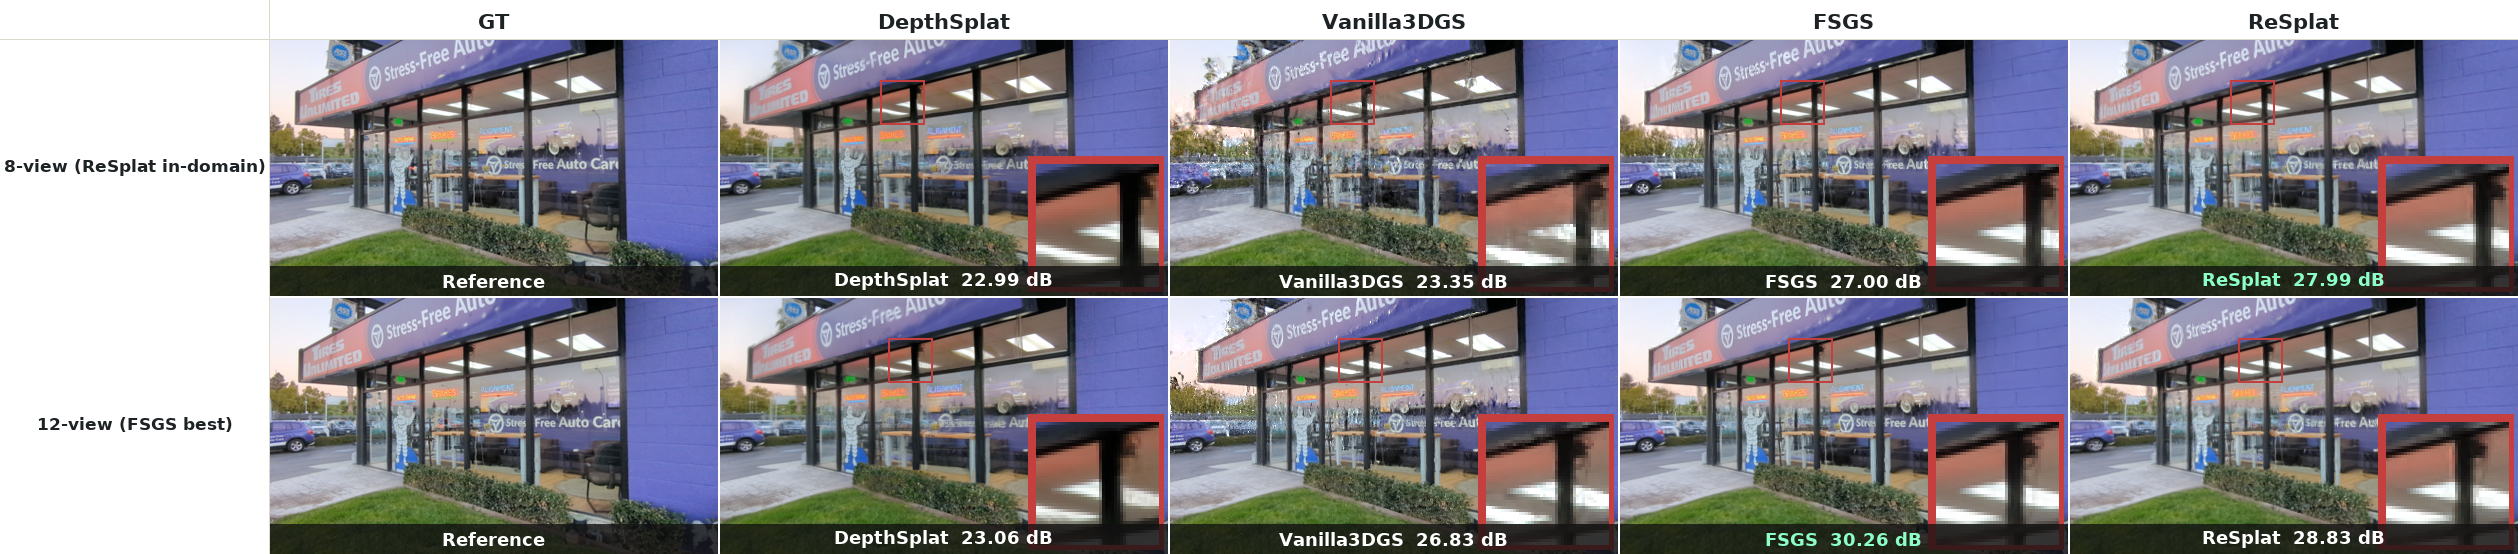
\includegraphics[width=\textwidth]{figures/qualitative_comparison_dl3dv_resplat.png}
\caption{DL3DV scene(§4.2 in-domain 체크포인트 매칭 원칙에 따라 DepthSplat/ReSplat 모두 이 데이터셋으로 학습된 체크포인트 사용)에서 GT/DepthSplat/Vanilla3DGS/FSGS/ReSplat 5개 방법 정성적 비교, budget=300\,s. 위 행은 8-view(ReSplat의 진짜 in-domain 지점, ReSplat이 27.99\,dB로 4개 방법 중 최고), 아래 행은 12-view(FSGS가 30.26\,dB로 최고). 확대 영역(빨간 박스)에서 DepthSplat의 구조물 경계 흐림이 가장 두드러지며, ReSplat은 같은 계보의 DepthSplat보다 뚜렷이 선명하지만 8-view에서도 FSGS와 근소한 차이, 12-view에서는 FSGS에 못 미친다 — 표~\ref{tab:resplat-exploratory}의 수치와 일관된다.}
\label{fig:qualitative-dl3dv-resplat}
\end{figure}
